%%%%%%%%%%%%%%%%%%%%%%%%%%%%%%%%%%%%%%%%%%%%%%%%%%%%%%%%%%%%%%%%%%%%%%%%%%%%%%%
%     enunciado.tex:    Enunciado de la práctica 2 de GIEAI-Informática
%%%%%%%%%%%%%%%%%%%%%%%%%%%%%%%%%%%%%%%%%%%%%%%%%%%%%%%%%%%%%%%%%%%%%%%%%%%%%%%

\documentclass[english,a4paper,11pt]{article}

\usepackage[latin1]{inputenc}  % codificación de caracteres de este archivo
\usepackage[spanish]{babel}    % Traducir: ``abstract'' ---> ``resumen''   etc.
\usepackage{fancyhdr}          % páginas con cabecera y pie
\usepackage{listings}          % listados de código fuente
\usepackage{float}             % para que los listados floten como las figuras
\usepackage{vmargin}           % ajuste de márgenes fácil de usar
\usepackage[T1]{fontenc}       % meter fuentes vectoriales
\usepackage{graphicx}          % figuras
\usepackage{upquote}           % comilla recta con \textquotesingle
\usepackage{placeins}          % orden \FloatBarrier para mantener figuras a raya

\usepackage[implicit=false]{hyperref}  % enlaces web (el parámetro implicit=false
                                       % evita problemas con el # de #include etc.)
                                       % uso explícito: \href[options]{URL}{text}
                                       %                \url{URL}

% mis abreviaturas
\newcommand{\C}{\texttt{C}}            % escribirá \C en lugar de \texttt{C}
\newcommand{\Pascal}{\texttt{Pascal}}  % idem con \Pascal ...
\newcommand{\fun}[1]{\texttt{#1()}}    % "\fun{main}" ---> "main()" en letra typewriter
\newcommand{\hex}[1]{\texttt{#1}$_{hex}$}
\newcommand{\bin}[1]{\texttt{#1}$_{bin}$}
\newcommand{\enesimo}{\mbox{n-ésimo}}
\newcommand{\muvision}{\textit{$\mu\!$Vision4}}
\newcommand{\keilmuvision}{\textit{Keil}~\muvision}
\newcommand{\codigo}[1]{\texttt{#1}}
\newcommand{\menu}[1]{\textit{#1}}

% Órdenes para alternar entre el estilo español (ligera separación extra
% entre párrafos) y el estilo por defecto (párrafos junticos junticos)
\newcommand{\parrafosjuntos}{\setlength{\parskip}{0pt}}
\newcommand{\parrafosseparados}{\setlength{\parskip}{1.5ex plus 0.6ex minus 0.5ex}}

% datos importantes del documento
\newcommand{\titulo}{Práctica 3: Herencia y sobrecarga en Java}     % <<--- TÍTULO
\newcommand{\fecha}{Semana de laboratorio 3}                         % <<--- TEMA
\newcommand{\asignatura}{Tecnología de Videojuegos}
\newcommand{\institucion}{UAH, Departamento de Automática, ATC-SOL}
\newcommand{\paginaweb}{http://atc1.aut.uah.es}

% portada
\title{\asignatura \\ \titulo}
\author{\institucion \\ \url{\paginaweb}}
\date{\fecha}

% márgenes un poco más finos
\setmargrb{25mm}{20mm}{25mm}{20mm}    % left, top, right, bottom

% encabezado y pie
\pagestyle{fancy}
\lhead{\footnotesize \parbox{11cm}{\asignatura}}
\lfoot{\footnotesize \parbox{11cm}{\institucion}}
\cfoot{}
\rhead{\footnotesize \titulo}
\rfoot{\footnotesize Página \thepage}
\renewcommand{\headheight}{24pt}
\renewcommand{\footrulewidth}{0.4pt}
%\renewcommand{\headrulewidth}{0pt}

% listados de código fuente flotantes
%\newfloat{floatlisting}{h}{}
%\floatname{floatlisting}{Listado}

% estilo de los listados de código
\lstset{numbers=left,                 % números de línea
        numberstyle=\tiny,            % tamaño de los num. de línea
        extendedchars=true,           % acentos, eñes...
        %frame=single,                 % marco que encuadra al listado
        basicstyle=\footnotesize\ttfamily,   % tipo de letra
        showstringspaces=false}       % no mostrar espacios de las cadenas

\graphicspath{{figs/}}                % ruta de las figuras

\begin{document} % ------------------ Aquí empieza el documento ----------------------

% redefinir el nombre de algunas cosas
\renewcommand{\tablename}{Tabla}                  % mejor "Tabla" que "Cuadro"
\renewcommand{\listtablename}{Indice de tablas}
% definidos originalmene en:
%/usr/share/texmf-texlive/tex/generic/babel/spanish.ldf

\maketitle              % montar el título aquí­ con los parámetros definidos arriba
\thispagestyle{empty}   % no poner número de página ni nada de nada en la 1ª página

\renewcommand{\abstractname}{}         % eliminar "Resumen"
\begin{abstract}                       % resumen (sin la palabra "Resumen")
\noindent \textbf{Objetivos:}
\begin{itemize}
\item Practicar el mecanismo de herencia en Java
\item Practicar la sobrecarga de métodos
\item Desarrollar buenos hábitos de programación
\item Comprender una jerarquía de clases utilizando un diagrama de clases en UML
\item Practicar los modificadores de acceso en Java
\item Practicar la utilización de paquetes
\item Afianzar la comprensión de POO
\end{itemize}
\end{abstract}

\sloppy              % hacer más flexible el cálculo del espacio entre palabras para
                     % evitar errores de tipo "overfull box"
                     % (lo contrario de \sloppy es \fussy)

\parrafosseparados   % separación entre párrafos (por defecto saldrán pegados)

\subsection*{Comentario inicial}
Se pretende desarrollar un videojuego RPG de fantasía medieval. El juego tendrá tres tipos de personaje (mago, guerrero o ladrón), cada uno con una serie de habilidades específicas. Así mismo, cada personaje podrá tener un arma (espada, arco o bastón). Como primer paso para el desarrollo del videojuego, se pretende crear una biblioteca de clases que modele los datos presentes en el juego e implemente la lógica de algunas acciones del mismo.

La práctica de programación recomendada es desarrollar las clases por separado, asegurando que cada una funciona correctamente de manera individual, para poco a poco ir integrándolas hasta obtener la aplicación final. Siguiendo esta lógica, realice los siguientes dos ejercicios.

\subsection*{Ejercicio 1}
El primer paso en el desarrollo del videojuego es la programación de las armas de los personajes. Para ello se partirá de una clase \texttt{Arma} que servirá como clase base para el resto de las armas. De \texttt{Arma} derivan tres clases más: \texttt{Espada}, \texttt{Arco} y \texttt{Baston}. 

\begin{figure}
  \centering
  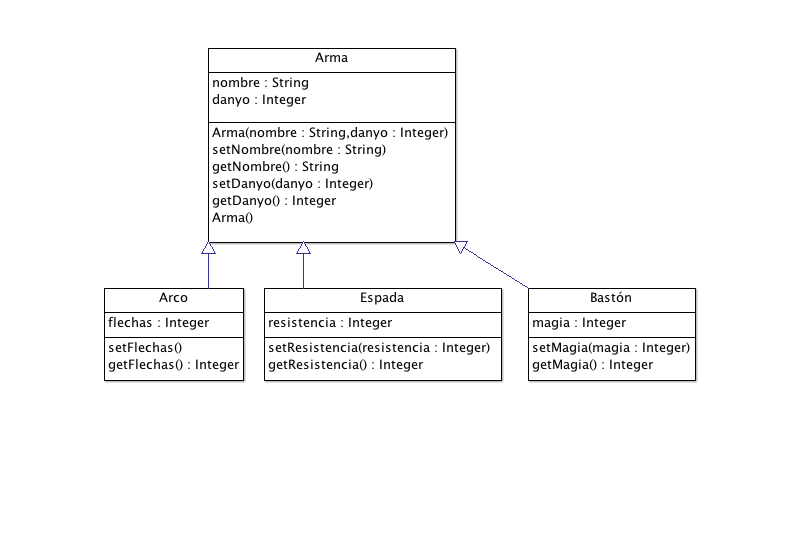
\includegraphics[width=0.9\textwidth]{figs/ej1}
  \caption{Diagrama de clases UML a implementar en el ejercicio 1}
  \label{fig:ej1}
\end{figure}

La figura~\ref{fig:ej1} representa el diagrama de clases que se pretende implementar. Hágalo siguiendo los siguientes pasos. Todas las armas tienen un nombre y un daño asociado, ambas guardadas, respectivamente, en los atributos \texttt{nombre} y \texttt{danyo}. Adicionalmente, cada arma guarda un dato específico a la misma, el arco contiene el número de flechas restante, la espada la resistencia de la misma, y el bastón puntos de magia.

Todos los atributos son protegidos mientras que todos los métodos son públicos. Los métodos get/set establecen o leen el valor del atributo respectivo.

\begin{enumerate}
\item Implemente la clase \texttt{Arma} dentro del paquete \texttt{p3.armas}. Compruebe su correcto funcionamiento instanciando la clase varias veces e ejecutando los métodos dentro de \texttt{main()}.
\item Implemente las clases \texttt{Espada}, \texttt{Arco} y \texttt{Baston} dentro del paquete \texttt{p3.armas}. Compruebe su correcto funcionamiento instanciando las clases varias veces e ejecutando los métodos dentro de \texttt{main()}.
\item Implemente los constructores apropiados de las tres clases anteriores. Suponga que por defecto el arco tiene 10 flechas, la espada 20 puntos de resistencia y el bastón 15 puntos de magia. Sugerencia: Utilice un constructor con una llamada explícita al construtor de la superclase por medio de la palabra reservada \texttt{super}.
\item Sobrecargue el método \texttt{toString()} en las cuatro clases anteriores de modo que, al ser invocado, devuelva una cadena describiendo la clase en cuestión con todos sus campos. Compruebe su correcto funcionamiento.
\item Cree un vector \texttt{Arma} conteniendo objetos de tipo \texttt{Espada}, \texttt{Arco} y \texttt{Baston}. Imprima, dentro de un bucle, la descripción de todos los objetos invocando \texttt{toString()} y verifique cómo funciona el polimorfismo.
\item Se quiere implementar un método \texttt{usar()}, presente en todas las clases, que imite la utización del arma. Su comportamiento cambia en función de la clase: En la clase \texttt{Arco}, debe reducir en uno el número de flechas, en \texttt{Espada} reduce la resistencia mientras que en \texttt{Baston} decrementa la magia. Piense qué habría que cambiar en la jerarquía de clases y discutalo con el profesor antes de implementarlo.
\item Implemente en método \texttt{estaDisponible()}, presente en todas las clases, que devuelve verdadero si el arma está disponible para el combate o falso en caso contrario. El arma esta disponible si el arco tiene flechas, la espada tiene puntos de resistencia, o el bastón tiene puntos de magia. Realice los cambios oportunos en el codigo.
\end{enumerate}

\subsection*{Ejercicio 2}
Una vez que se han implementado las clases con las armas del juego, se pretende programar las clases que representan a los personajes. Pueden ser tres: Mago, guerrero y ladrón. Cada personaje tendrá un arma y podrá luchar con otros personajes. 

\begin{figure}
  \centering
  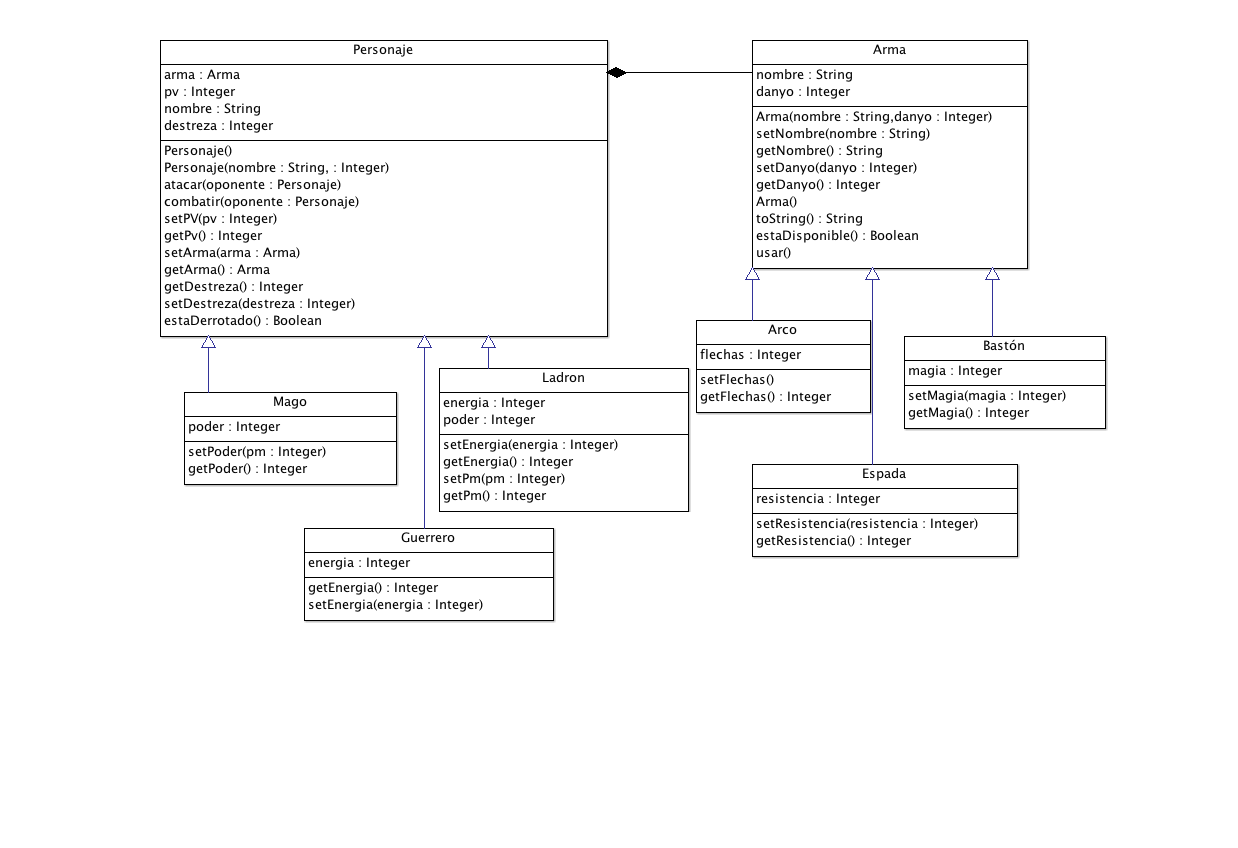
\includegraphics[width=\textwidth]{figs/ej2}
  \caption{Diagrama de clases UML a implementar en el ejercicio 2}
  \label{fig:ej2}
\end{figure}

La figura 2 muestra el diagrama de clases completo a implementar. Hágalo siguiendo los siguientes pasos.

\begin{enumerate}
\item Implemente la clase \texttt{Personaje} dentro del paquete \texttt{p3.personajes}, a excepción de los métodos \texttt{atacar()} y \texttt{luchar()}. El método \texttt{estaDerrotado()} devuelve \texttt{true} si el personaje tiene cero o menos PV.
\item Implemente las clases \texttt{Mago}, \texttt{Guerrero} y \texttt{Ladron}, a excepción de los métodos \texttt{atacar()} y \texttt{luchar()}. Por defecto, el mago tendrá un bastón, el ladrón un arco y el guerrero una espada, téngalo en cuenta a la hora de programar el constructor. Sugerencia: Utilice una llamada al constructor de la superclase por medio de \texttt{super}.
\item Sobrecargue el método \texttt{toString()} en las cuatro clases anteriores para poder visualizar el contenido de los atributos fácilmente.
\item El mecanismo de combate es el siguiente. Un combate es una sucesión de ataques, primero ataca quien inicia el combate, después contrataataca el oponente, y así sucesivamente. El combate comienza invocando al método \texttt{combatir()}, cada combatiente ataca por turnos hasta que uno se queda sin PV, en cuyo caso se encuentra derrotado. El ataque se realiza invocando al método público \texttt{atacar()}; al invocarse este método se restará a los PV de cada personaje el daño del arma del personaje contrario más su destreza. Después de cada ataque el mago pierde un punto de poder, el guerrero un punto de energía y el ladrón un punto de energía o poder. Si se agota cualquiera de esos elementos la destreza no suma al daño ocasionado por el personaje. Análogamente, si el arma no está disponible (arco sin flechas, espada dañada o bastón sin magia), no se suma al daño el efecto del arma.  En cada ataque se invocará el método \texttt{usar()} del arma para que actualice su estado. Implemente los métodos \texttt{combatir()} y \texttt{atacar()}.
\end{enumerate}

\end{document} 
